\section{Stacking}
Stacking is a machine learning technique that involves training a second-level model to make predictions based on the outputs of several base models. It is a form of ensemble learning, which combines the predictions of multiple models to create a more accurate and stable prediction.
\\\\
In stacking, the base models are trained on the same dataset and then make predictions. These predictions are then combined and used as input to the second-level model, which is trained to make a final prediction based on the output of the base models. This final prediction is typically more accurate than the predictions of the individual base models.
\\\\
Stacking can be used with a variety of base models, such as decision trees, neural networks, or support vector machines. It is a powerful technique that can improve the performance of machine learning models, especially when the base models have complementary strengths and weaknesses.

\begin{figure}[H]
    \centering
    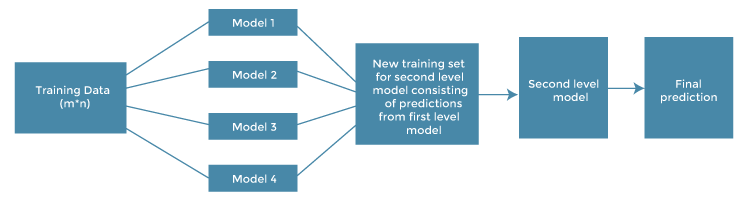
\includegraphics[width=.7\textwidth]{figs/stacking.png}
    \caption{Stacking schematic}
    \label{fig:stacking}
\end{figure}

In our case, we implemented a stacking regressor in the \verb|stacking.py| file. Our ensemble regressor gets his base approximations from all the approximations discussed here above (except random forests and neural networks). The second level model is based on a decision tree. All first level models are trained with the tuned hyperparameters for each zone. Here are the results we obtained :

\begin{table}[H]
\centering
\begin{tabular}{|c|c|c|}
\hline
         & MSE      & MAE      \\ \hline
Stacking & 0.070009 & 0.194127 \\ \hline
\end{tabular}
\caption{Results for stacking regressor}
\label{tab:stacking}
\end{table}

As can be seen in the table here above, the results we obtained using stacking were an improvement on the individual regression algorithms but were still unable to beat the random forests and neural networks.